% 4  Results
% 4.1  Various plots with differing initial waves and bays ? including top-down view
% 4.1.1  Plots of same initial wave through different bays
% 4.1.1.1  Discuss resonance in terms of max. run up vs. max run up in plane-shaped bay (very large m)
% 4.1.1.1.1  Also in terms of how far up shore wave travels (top-down view)
% 4.1.2  Include at least one plot of eigenfunctions in both physical and sigma space
% 4.1.3  Include error in x wall mentioned previously in all different plots
% 4.2  Comparison to Pelinovsky?s analytic solution for m=2 and initial profile from paper
% 4.2.1  Comparison to initial condition
% 4.2.2  Alter number of eigenvalues, sigma (or x) steps, and lambda steps (each separately) to see what it takes to converge to analytic solution.
% 4.3  Possibly use max. run up and min. run down as a convergence metric - when varying number of eigenvalues, sigma (or x) steps, and lambda steps - for other values of m
% 4.4  Show how closely nonlinear system follows superposition principle ? measure of how linear/nonlinear the system is

\section{Results}
	
	\graphicspath{{section/Res/}}
	



\begin{frame}
		\frametitle{IC}
		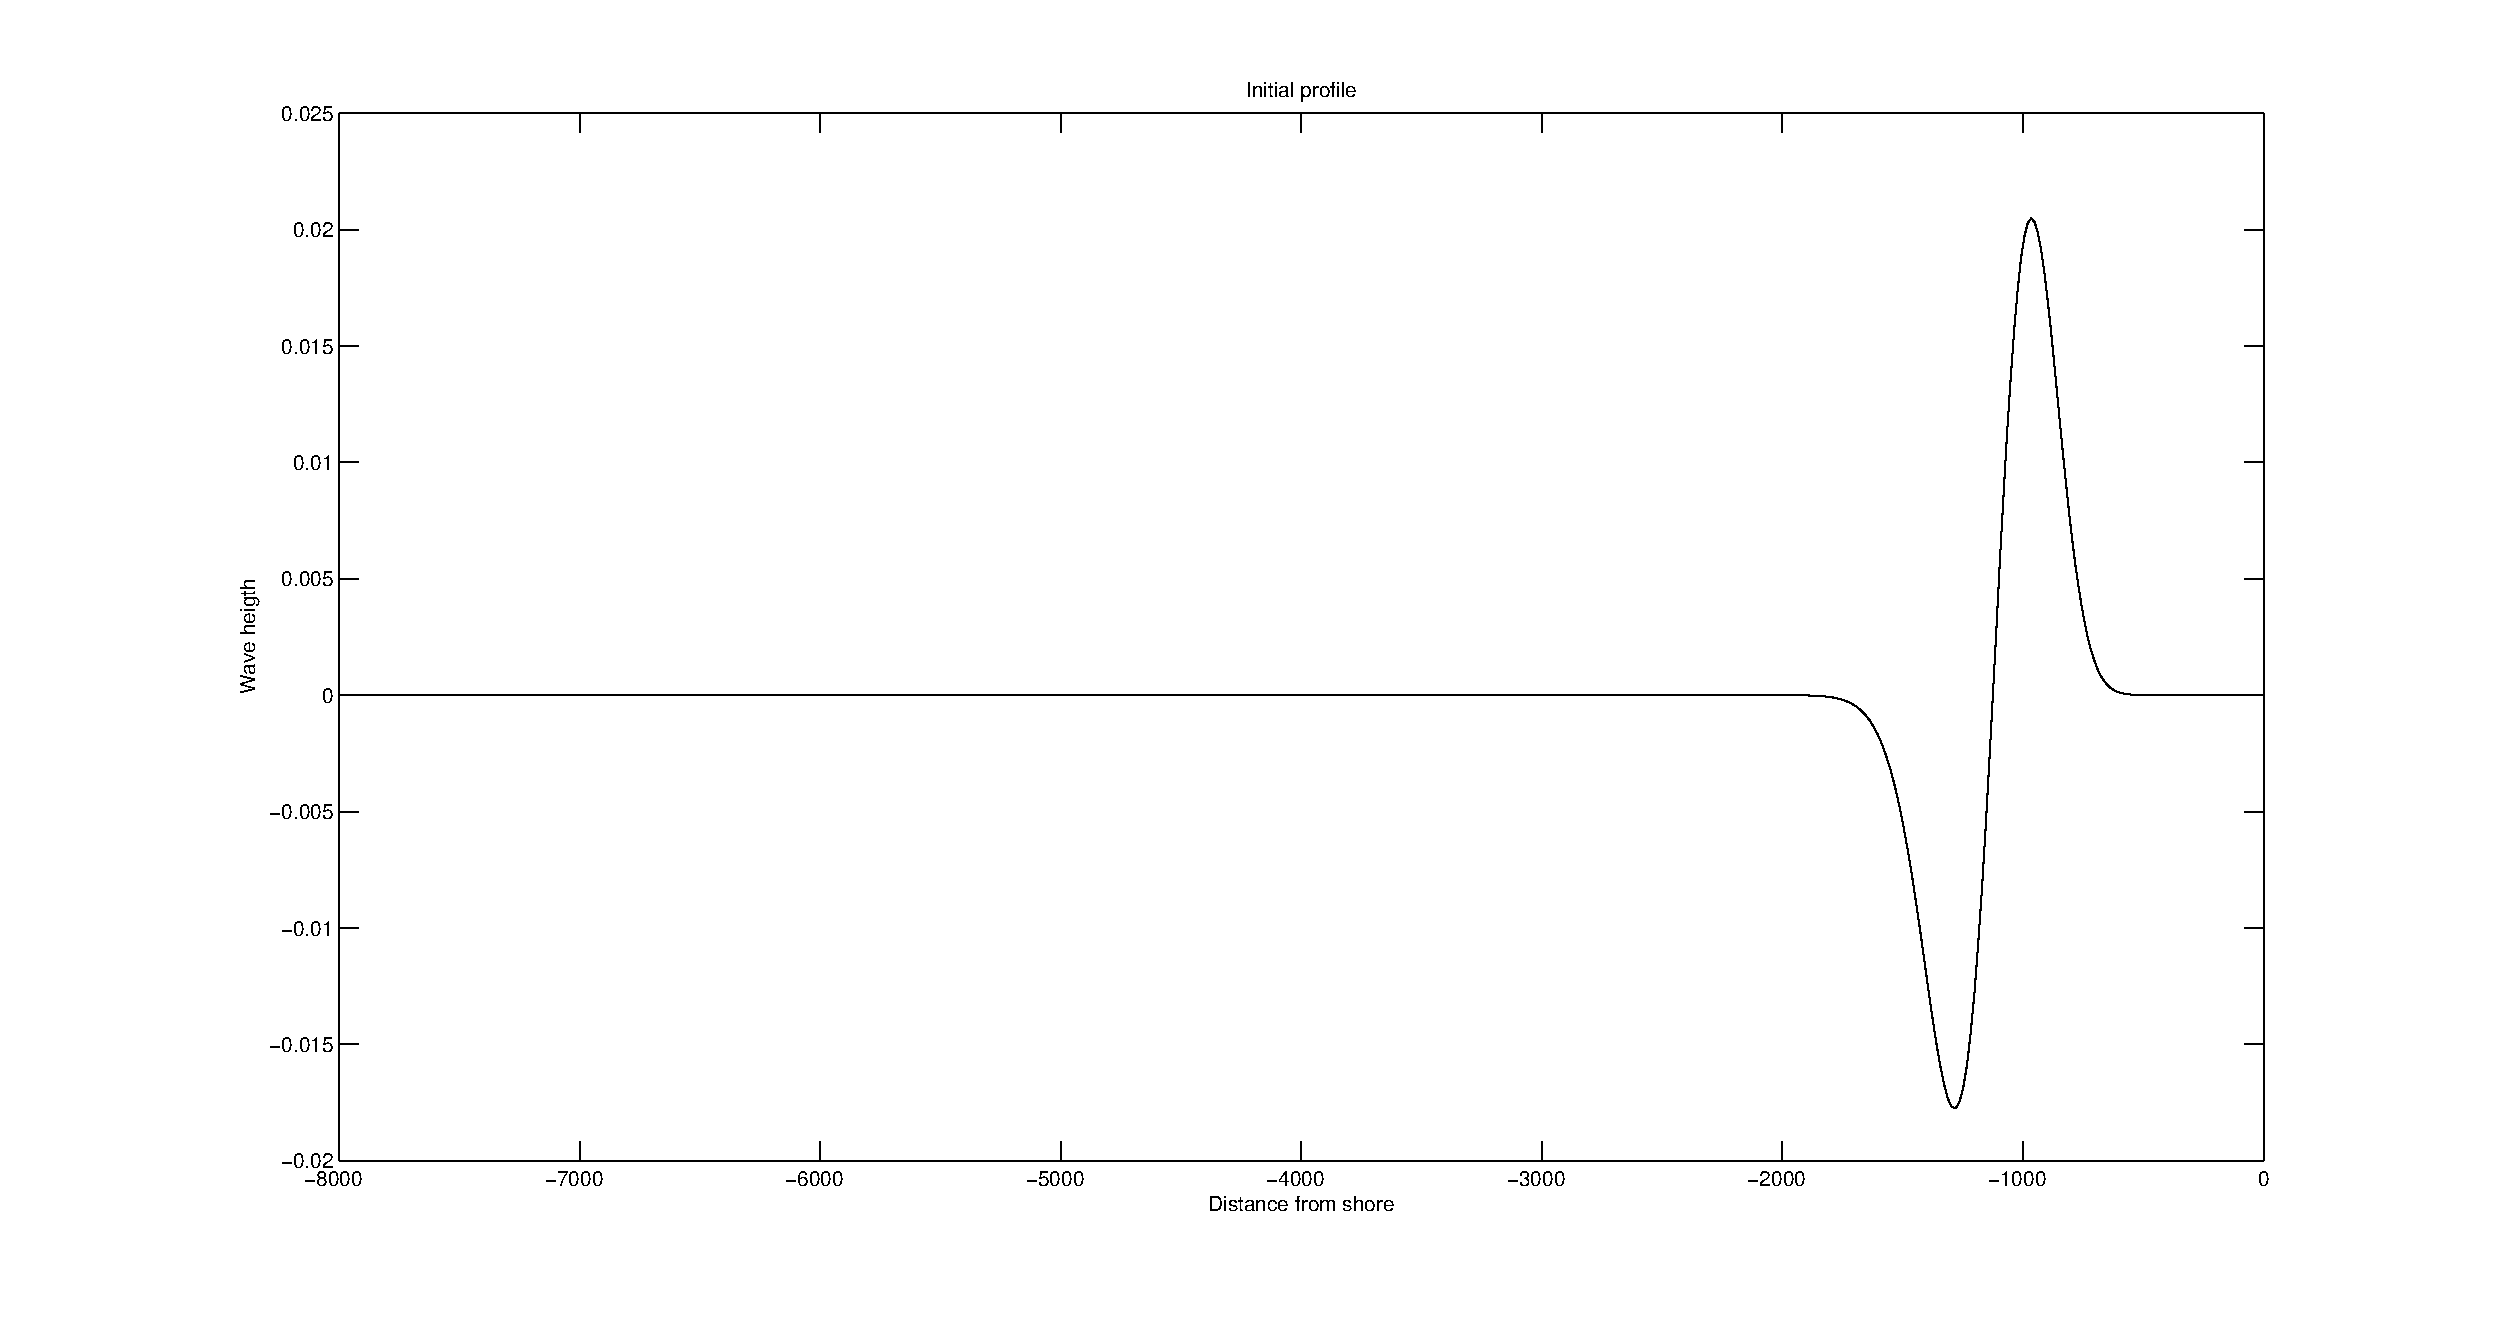
\includegraphics[width=\textwidth]{IC.eps}
		\end{frame}

\begin{frame}
		\frametitle{Eigen values}
		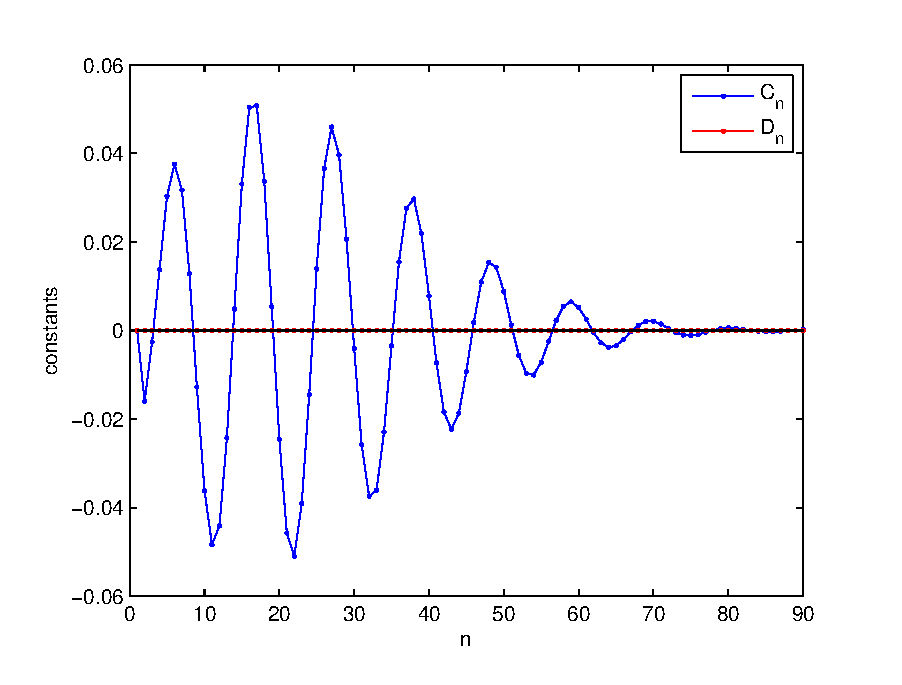
\includegraphics[width=\textwidth]{Const.eps}
		\end{frame}

	
	
				\begin{frame}
		\frametitle{Eigen Functions}
		\begin{tabular}{|c|c|}\hline
		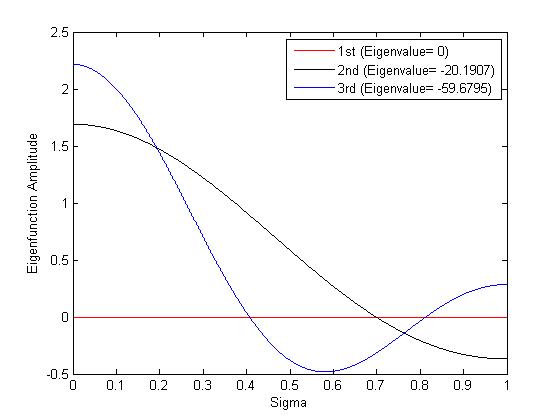
\includegraphics[width=.45\textwidth]{Eigenfunctions1.png}&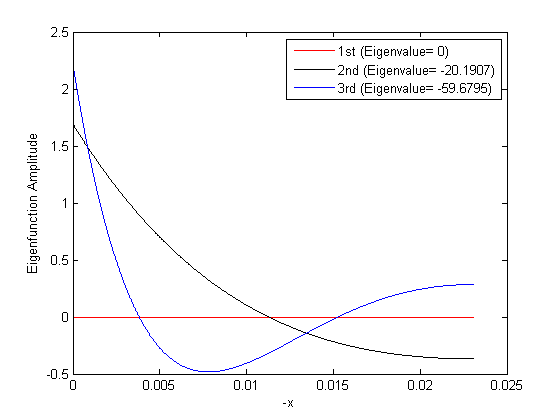
\includegraphics[width=.45\textwidth]{Eigenfunctionsx1.png}\\\hline
		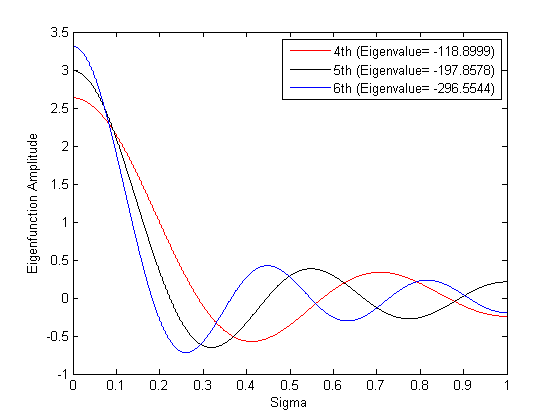
\includegraphics[width=.45\textwidth]{Eigenfunctions2.png}&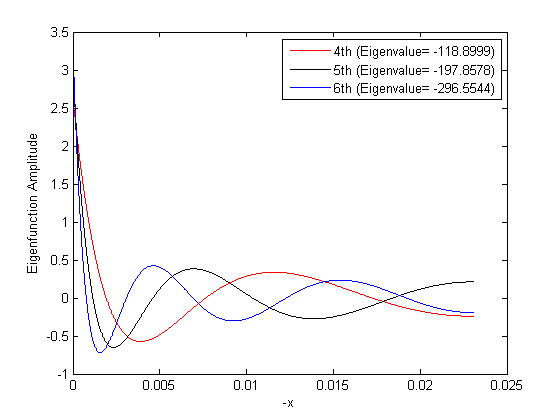
\includegraphics[width=.45\textwidth]{Eigenfunctionsx2.png}\\\hline
		\end{tabular}
		
	\end{frame}
	
	
	
	
		
	\begin{frame}
		\frametitle{Numerical error in max run-up}
		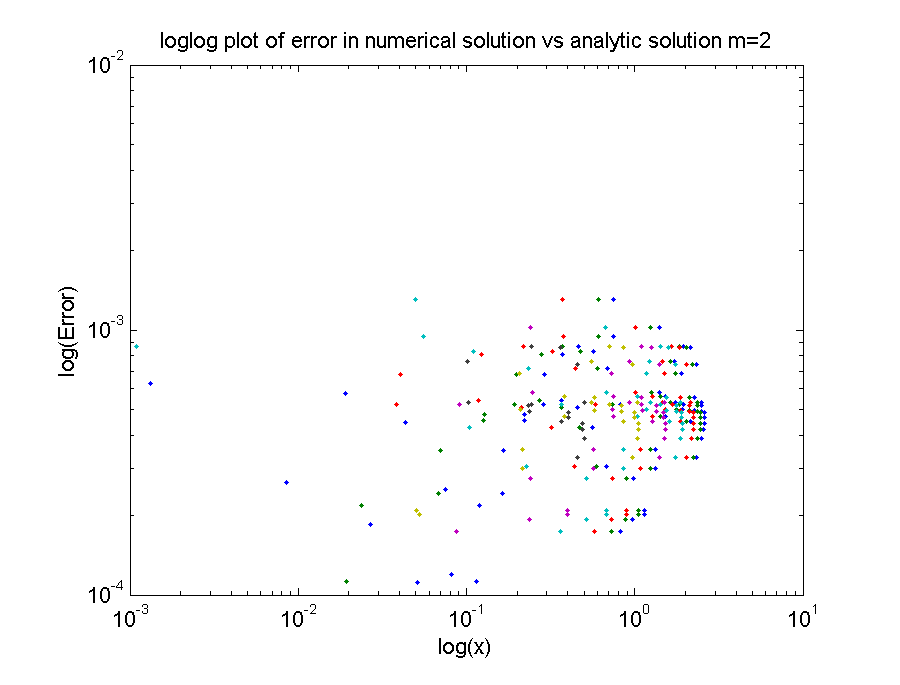
\includegraphics[width=\textwidth]{Error.eps}
		
	\end{frame}
	
	
	\begin{frame}
		\frametitle{Error in boundary assumption}
		\centering
		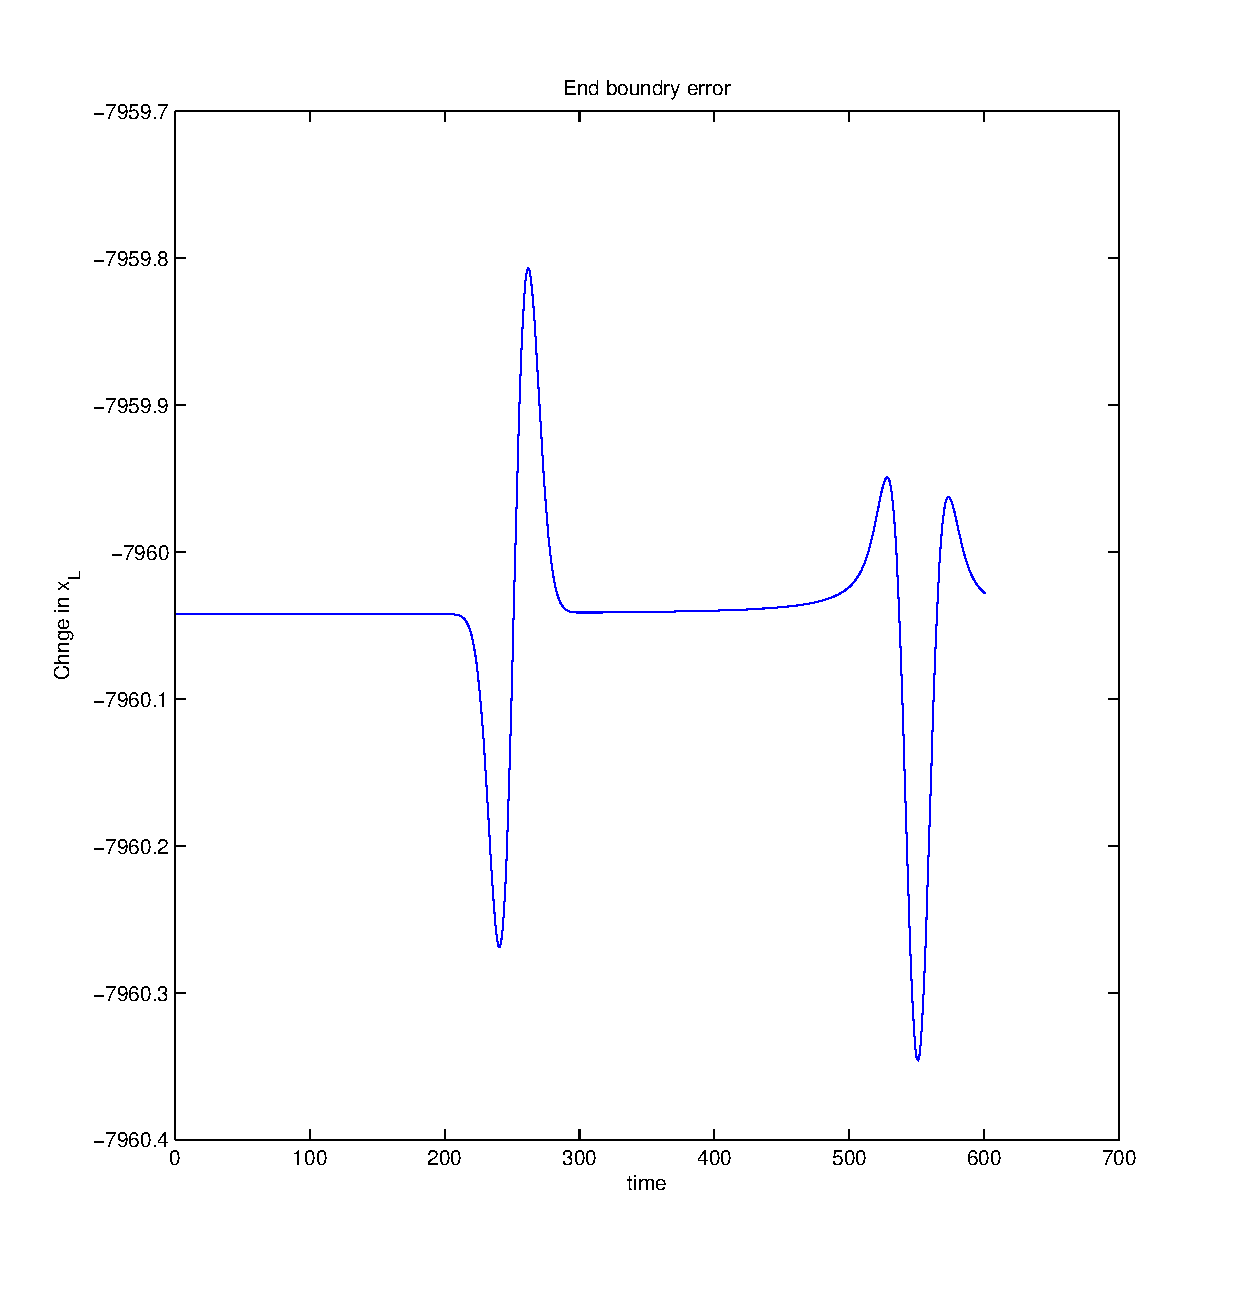
\includegraphics[width=.7\textwidth]{x_l.eps}
		
	\end{frame}
	
	
	
	
		\begin{frame}
		\frametitle{Effect of $m$ on run-up}
		\centering
		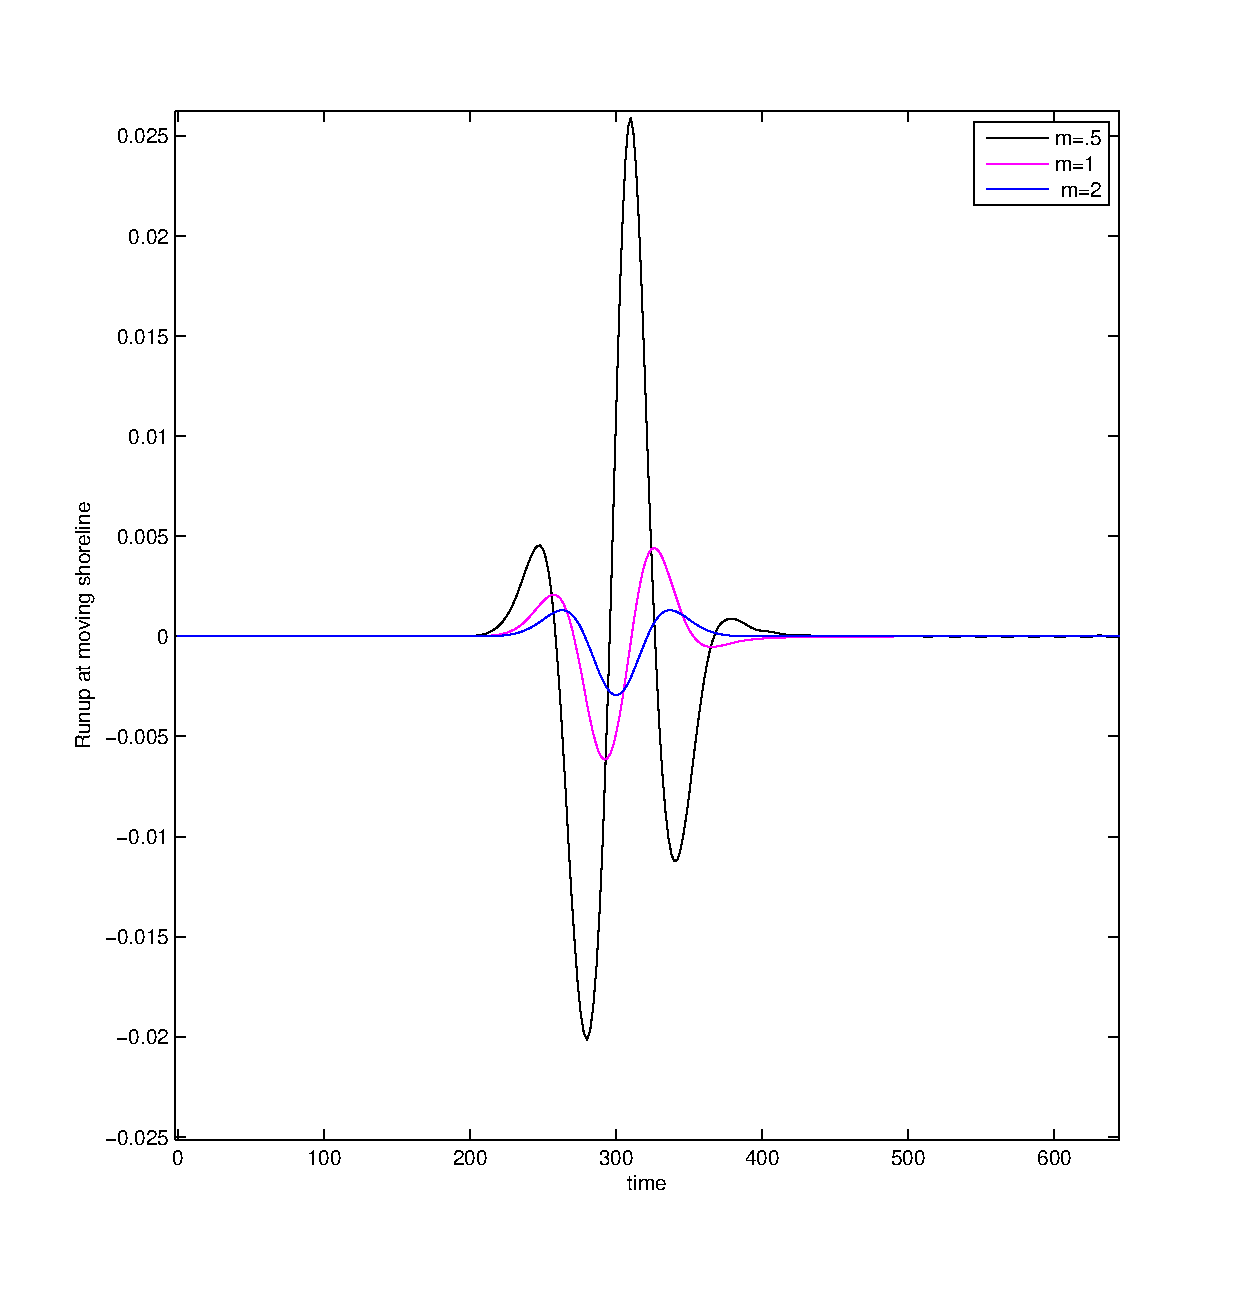
\includegraphics[width=.7\textwidth]{Runup.eps}
		
	\end{frame}
	
			\begin{frame}
		\frametitle{Effect of $m$ on run-up 2}
		\centering
		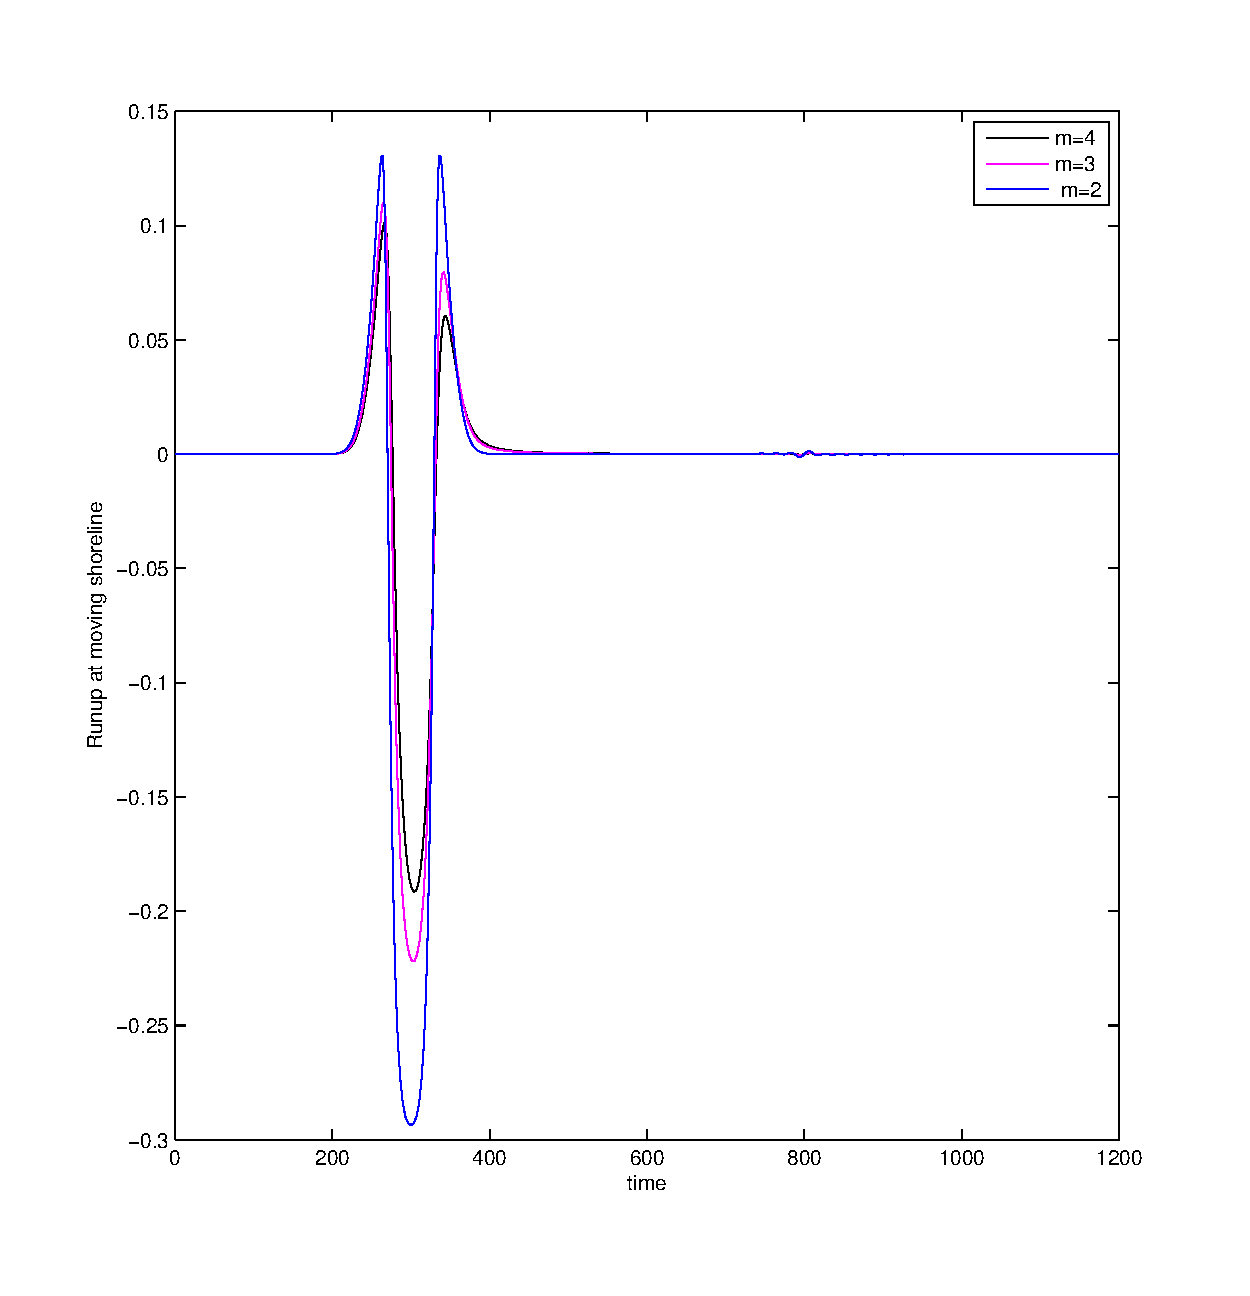
\includegraphics[width=.7\textwidth]{Runup2.eps}
		
	\end{frame}
	
